\chapter{Úvod do problematiky}\label{chap:issues_overview}

V tejto úvodnej kapitole si popíšeme a vysvetlíme základné pojmy, ktorých znalosť je nevyhnutná v našej práci. Vysvetlíme si ako funguje počítačové videnie, objektová detekcia, konvolučné neuronové siete a taktiež sa zameriame na výskum objektovej detekcie pri malej trénovacej množine (Few shot object detection), ktorý budeme chcieť využiť v našej práci pre učenie nových objektov aj z veľmi malého množstva dát.

\section{Počítačové videnie}


\setlength{\parindent}{20pt}

\hspace{\parindent}Počítačové videnie je súčasnej dobe veľmi rastúci a progresívny smer v informatike. Snaží sa priblížiť vnímaniu sveta z pohľadu ľudského oka, ktoré je pre nás prirodzené a automaticky sme schopný rozpoznávať objekty, farby a kontext toho čo vidíme. Avšak plné sémanticke pochopenie videnej reality je veľmi komplexné a zatiaľ nie sme schopný ho získať spracovaním digitálneho obrazu. Hlavne preto, že pochopenie obrazu môže vyplývať zo súvislostí, ktoré nie sú súčasťou obrazu.

Avšak počítačové videnie sa posúva veľmi rýchlo vpred. Neustále vynikajú nové algoritmy a prístupy či už na detekciu objektov alebo klasifikáciu obrazu. Medzi základné problémy počítačového videnia patrí klasifikácia, objektová detekcia a segmentácia. Pri klasifikácii sa snažíme obraz priradiť do jednej z tried. V objektovej detekcii sa snažíme v obraze určiť oblasti všetkých známych objektov a priradiť ich do tried. A pri segmentácii je našim cieľom rozdeliť obraz do viacero oblastí, každému pixlu určiť oblasť do ktorej patrí. 

\section{Príznaky}

\hspace{\parindent}Pri riešení problémov v počítačovom videní sa využívajú príznaky. Príznak v počítačovom videní je meratelný kus dát v obrázku, ktorý je unikátny pre špecifický objekt. Príznak môže reprezentovať napríklad štýl sfarbenia, nejaký tvar, či už čiaru alebo hranu v obraze alebo nejakú časť obrazu. Vďaka dobrému príznaku dokážeme od seba rozlíšiť objekty. Napríklad ak máme rozlíšiť mačku a bicykel tak ako dobrý príznak by mohlo byť, že na obrázku sa nachádza koleso. Hneď by sme vedeli vďaka tomuto príznaku klasifikovať obrázok do týchto dvoch tried. Ak by sme však mali za úlohu zistiť či je na obrázku motorka alebo bicykel, tak by nám tento príznak veľmi nepomohol a museli by sme pozerať na iné príznaky. Preto zväčša neextrahujeme z obrázku len jeden príznak, ale pre lepšiu detekciu vyberáme viacej príznakov, ktoré tvoria príznakový vektor. 

Nie je presná definícia aké príznaky obrázku by sme mali použiť, ale závisí to skôr od nášho cieľu a typu úlohy. Príznaky sa delia na lokálne a globálne. Globálne príznaky sú také, ktoré platia pre celý obrázok. Napríklad ako ako veľmi sú dominantné jednotlivé farby v obrázku. Globálny príznak nám opisuje obraz ako celok a mal by reporezentovať nejakú jeho špecifickú vlastnosť. Lokálne príznaky sa extrahujú len z určitej zaujímavej oblasti v obrázku, využivajú sa najmä pri objektovej detekcii. Najskôr nájdeme zaujímavé oblasti, ktoré by mohli reprezentovať nejakú zaujímavú vlastnosť alebo nejaký objekt. Následne vytvoríme príznakový vektor pre danú oblasť, ktorý by nám mal poskytnúť zásadnú informáciu o tejto časti obrazu. Treba rátať s tým, že objekt na obrázku môže byť rôznej veľkosti, rôzne natočený, rôzne osvetlený, zašumený, môže sa nachádzať v rôznych častiach obrázku a podobne. Preto naše príznaky by mali byť čo najviac odolné voči týmto zmenám(mali by ich čo najmenej ovplyvňovať). Čím viac invariatné príznaky voči týmto zmenám si zvolíme tým lepšia je naša detekcia. 

\section{Objektová detekcia}

\hspace{\parindent}Asi najskúmanejším problémom v počítačovom videní je objektová detekcia, ktorá spočíva v rozpoznaní jednotlivých objektov a ich pozícii v digitálnom obraze. Dá sa k tomuto problému pristupovať rôznymi spôsobmi, dá sa pristupovať k tomuto problému tradičnými metódami počítačového videnia, alebo dnes už veľmi rozšireným s oveľa lepšími a presnejšími výsledkami, ako pri tradičných metódach a to pomocou hlbokého učenia, ktorých klúčom je naučiť sa na veľkých dátach extrahovať príznaky tak aby mala detekcia čo najväčšiu presnosť.

\subsection{Tradičé metódy}
\hspace{\parindent}Tradičné metódy v objektovej detekcii majú zvyčajne tri etapy: vybratie oblasti, extrakcia príznakov, klasifikácia objektu. 

V prvej etape sa snažíme lokalizovať objekt. Keďže objekt môže byť rôznej veľkosti, musíme skenovať celý obrázok pomocou posúvneho okna rôznej veľkosti. Táto metóda je výpočtovo náročná. 

V druhej etape použijeme použijeme metódy ako SIFT, HOG na extrakciu vizuálnych príznakov na rozpoznanie objektu. Tieto príznaky nám poskytujú sémantickú a robustnú reprezentáciu. Avšak kvôli rôznemu osvetleniu, pozadiu a ulhu pohľadu je veľmi náročné manuálne navrhnúť deskriptor príznakov, ktorý by dokonale opísal všetky typy objektov. 

V treťej fáze klasifikácie objektu používame zväčša Support Vector Machine(SVM) alebo Adaboost pre klasifikáciu cieľových objektov zo všetkých kategórii aby bola reprezentácia viac hierarchická, sémantická a informatívnejšia pre vizuálne rozpoznávanie. 

Problémom pri tradičných metódach je výpočtová náročnosť pri generovaní kandidátov na bouning box (obdĺžnik ohraničujúci objekt) pomocou techniky posúvneho okna a taktiež manuálne nastavenie extrakcie príznakov nie je vždy veľmi presné. 

Medzi najznámejšie tradičné metódy objektovej detekcie patrí napríklad Viola Jones.

Viola Jones metóda vznikla už v roku 2001, bola veľmi využívana najmä na detekciu tváre vo fotoaparátoch a využívva sa do dnes. Stala sa populárnou vďaka jej presnosti a rýchlosti. Používa jednoduché príznakové klasifikátory, ktoré môžu byť rýchlo vypočítané porovnaním intenzity pixelov v malých regiónoch obrázku. Metóda využíva integrálny obrázok, čo robí výpočet týchto príznakov veľmi rýchly. Rýchlosť tejto metódy spočíva aj v rýchlom zamietnutí objektu v danej lokalite obrázku hned ako jeden z množiny jednoduchých príznakov bude zamietnutý a nasledujúci sa už v danej lokalite netestuje. 
\cite{viola2001rapid}


\begin{figure}
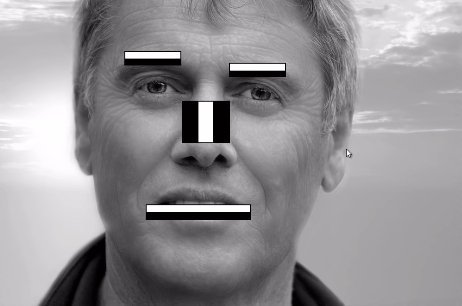
\includegraphics{images/viola_jones.jpg}
\caption{Ukážka detekcie jednoduchých príznakov vo Viola Jones}
\label{fig:image}
\end{figure}


\subsection{Konvolučné neuronové siete}

\subsubsection{Úvod do CNN}
\hspace{\parindent} Konvolučné neuronové siete (CNN) sú typ umelej neurónovej siete, ktorý v posledných rokoch zmenil oblasť počítačového videnia. 
Inšpirované spôsobom akým zraková kôra spracováva informácie, sú konvolučné neurónové siete špeciálne vhodné na analýzu údajov, ktoré majú mriežkovú štruktúru, ako napríklad obrázok. Sú schopné sa automaticky učiť príznaky z dát, miesto toho aby sme museli manuálne určiť extrakciu príznakov. Dosahujú vynikajúce výsledky na širokom spektre úloh, vrátane klasifikácie obrázkov, objektovej detekcie a segmentácie. 

\subsubsection{Konvolučné vrstvy}
\hspace{\parindent} Kľučovým stavebným blokom CNN je konvolučná vrstva, ktorá aplikuje rad filtrov na vstupné údaje, aby extrahovala relevantné príznaky. Každý filter je malá matica váh, ktorá je aplikovaná na lokálny región vstupu, a výstup konvoúcie je nová príznakova mapa, ktorá v sebe kóduje prítomnosť niektorých príznakov vo vstupných dátach. 

Napríklad, ak dostaneme na vstupe obrázok a naše filtre sú dizajnované na detekciu hrán, výstupná mapa príznakov zvýrazní umiestnenia hrán v obrázku. Filtre sú zväčša invariantné voči pohybu, čo znamená, že rozpoznajú príznak nezávisle od jej umiestnenia v obrázku. 

Viacero filtrov sa môže aplikovať na vstupný obrázok na extrakciu rôznych typov príznakov a výstup konvolučnej vrstvy je vicero príznakových máp, jedna pre každý filter. Počet a veľkosť filtrov sú hyperparametre, ktoré sa môžu nastaviť podľa potreby. 

\begin{figure}
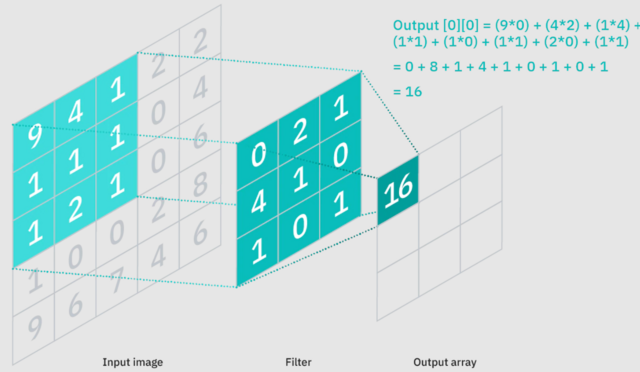
\includegraphics{images/CNN-layer.resized.png}
\caption{Ukážka konvolučnej vrstvy}
\label{fig:image}
\end{figure}

\subsubsection{Poolingové vrstvy}
\hspace{\parindent} Po konvolučnej vrstve sa v CNN zvyčajne nachádza poolingová vrstva, ktorá zmenšuje veľkosť dát, znižuje dimenziu a predchádzame vďaka nej overfittingu(pretrénovaniu). Poznáme niekoľko typov poolingu, vrátane max poolingu a average poolingu, ale najbežnejším je max pooling, ktorý vezme maximálnu hodnotu každého poolingového regiónu. 

Napríklad, ak pooling region je mriežka 2x2, max pooling vezme najväčšiu zo 4roch hodnôt v mriežke a vráti ju ako jednu hodnotu do výstupnej príznakovej mapy. Toto spôsobí redukciu veľkosti príznakovej mapy a ponecháme len najdôležitejšie príznaky. 

\subsubsection{Plne prepojené vrstvy}
\hspace{\parindent} Ďalej po konvolučných a poolingových vrstvách, CNN zvyčajne obsahujú jednu alebo viac plne prepojených vrstiev, ktoré kombinujú príznaky extrahované konvolučnými a poolingovými vrstvami na určenie finálnej predikcie. 

Plne prepojená vrstva je zvyčajne výstupná vrstva, ktorá vracia finálnu predikciu CNN. Počet neurónov vo výstupnej vrstve zavisí od tasku, ktorý máme. Napríklad, pre klasifikáciu obrázku, výstupná vrstva môže mať jeden neurón pre každú triedu, a neurón s najvyššou aktivačnou hodnotou by predstavoval predikovanú triedu. 

\subsubsection{Aktivačné funkcie a regularizácia}
\hspace{\parindent}Za účelom zavedenia ne-lineárnosti do modelu zvyčajne CNN obsahujú aktivačné funkcie v konvolučných a plne prepojených vrstvách. Najbežnejšou aktivačnou funkciou je Rectified Linear Unit (ReLU), ktorá má formu f(x) = max(0,x). Používajú sa aj iné aktivačné funkcie ako napríklad sigmoid a tanh. 

Na prevenciu overfittingu a zlepšenie generalizácie, konvolučné neurónové siete využívajú regularizačné techniky ako napríklad dropout, ktorý náhodne nastaví niektoré aktvácie v plne prepojených vrstvách na nulu počas tréningu. Toto spôsobuje zníženie komplexnosti modelu a núti zvyšné neuróny učiť sa robustnejšie príznaky. 

\begin{figure}
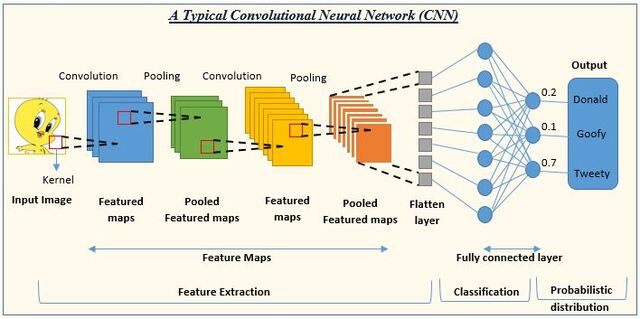
\includegraphics{images/CNN.resized.JPG}
\caption{Ukážka príkladu CNN}
\label{fig:image}
\end{figure}

\subsubsection{Tréning CNN}
\hspace{\parindent}Tréning CNN zahŕňa prispôsobenie váh filtrov a spojení v sieti na minimalizovanie stratovej funkcie, ktorá meria rozdiel medzi predikciou a skutočným labelom. Process trénovanie CNN môže byť rozdelený na nasledovné kroky:

Prvým krokom je vyzbierať anotovaný dataset, ktorý bude použitý na trénovanie modelu. Tento dataset by mal byť dostatočne veľký a rôznorodý aby sa vedel generalizovať na nové obrázky. Pred tréningom modelu, je zväčša nevyhnutné predspracovanie dát, aby sme sa uistili, že sú vhodné pre CNN. To môže zahŕňať prispôsobenie veľkosti obrázkov alebo augmentáciu dát aplikovaním náhodných transformácii, pre rôznorodosť datasetu a predchádzaniu overfittingu. 

Ďalším krokom je rozdelenie datasetu na treningovú, validačnú a testovaciu množinu. Trénovacia množina je použitá na trénovanie CNN, validačná na vyhodnotenie CNN počas tréningu a testovacia na vyhodnotenie modelu po tréningu. Validačná množina je nápomocná pre nastavenie hyperparametrov CNN ako napríklad learning rate. Testovacia množina nám poskytuje približnú schopnosť generalizácie našej siete. 

Tretím krokom je definovanie CNN, čo obnáša výber počtu a typu vrstiev, veľkosť filtrov, výber aktivačných funkcií a ostatných hyperparametrov. Je veľa spôsobov ako nadizajnovať CNN, ktoré majú vplyv na jej výkon. Najlepšie je vyskúšať rôzne hyperparametre a architektúry CNN pre nájdenie najlepšej kombinácie k danému tasku. 

Ďalším krokom je určenie stratovej funkcie a optimalizačného algoritmu. Existuje veľa rôznych stratových funkcií, ktoré môžu byť použité, voľba stratovej funkcie záleží na tasku. Napríklad pre binárnu klasifikáciu môže byť použitý binary cross-entropy loss, kým pre klasifikáciu do viacerých tried môže byť použitá categorical cross-entropy loss. 
´
Optimalizačný algoritmus je zodpovendný za prispôsobenie váh siete na minimalizovanie stratovej funkcie. Njabežnejší optimaizačný algoritmus je stochastic gradient descent (SGD), ktorý je založený na gradiente stratovej funkcie vzhľadom na váhy. Iné často používané optimalizačné algoritmy sú napríklad Adam alebo RMSprop. 

Po tom ako určíme stratovú funkciu a optimalizačný algoritmus, CNN môže byť trénovaná iteratívnym aplikovaním optimalizačného algoritmu na tréningovú množinu a upravovaním váh siete. Optimalizačný algoritmus prispôsobí váhy v smere aby redukoval stratu a cieľom je nájsť váhy, ktoré dosahujú najnižšiu stratu. 

Počas tréningu je bežné rozdeliť trénovaciu množinu na mini-batche a aplikovať optimalizačný algoritmus postupne pre každý mini-batch zvlášť. Toto umožňuje upravovať váhy častejšie a často môže viesť k rýchlejšej konvergencii. 

Po trénovaní CNN je dôležité vyhodnotiť výkon na testovacej množine. Testovacia množina by mala byť dostatočne veľká aby nám ponkla spolahlivé vyhodnotenie nášho modelu a nemala by byť použitá pri tréningu. 

Výkon CNN môže byť vyhodnotený pomocou rôznych metrík. Zavisí od tasku, ktorú metriku je pre nás vhodné použiť.

\section{Few-shot object detection(FSOD)}
\hspace{\parindent}Problémom pri vačšine algoritmov objektovej detekcie je, že vyžadujú veľký dataset anotovaných obrázkov na tréning modelu, čo môže byť drahé a časovo náročné. 

Few-shot object detection je varianta objektovej detekcie, ktorá sa snaží učiť z malého datasetu. Je to inšpirované few-shot learningom, čo je typ strojového učenia, ktorý sa učí na malých trénovacích dátach. Few-shot learning si získal v posledných rokoch veľa pozornosti, vďaka jeho schopnosti adaptovať sa novým taskom s malým množstvom dát, čo je dôležité v prípade, že nemáme dostatok anotovaných dát. 

Few-shot object detection je náročný problém, pretože model sa musí naučiť chrakteristiky objektov z malého množstva príkladov, čo je náročné vzhľadom na komplexnosť a rôznorodosť objektov. Naviac model musí rozpoznať nové triedy, ktoré neboli videné počas tréningu, čo vyžaduje dobré rozlišovanie medzi odlišnými triedami. 

Napriek náročnosti, je to dôležitý problém, pretože má potenciál výrazne znížiť počet anotovaných dát potrebných na objektovú detekciu. 


\subsection{Prístupy k FSOD}
\hspace{\parindent}Sú viaceré prístupy, ktoré boli navrhnuté na FSOD, môžu byť zhrnuté do troch hlavných kategórií: meta-learning, transfer learning a augmentácia dát.

\subsubsection{Meta-learning}
\hspace{\parindent}Meta-learning je prístup, ktorý sa snaží naučiť sa učiť. Sústredí sa na trénovanie modelu, ktorý sa vie rýchlo prispôsobiť novým úlohám iba vďaka veľmi malému počtu obrázkov. Tento prístup zvyčajne zahŕňa trénovanie modelu, ktorý sa vie učiť z malého počtu dát buď použitím vonkajšej pamäti alebo optimalizačného algoritmu. Napríklad Model-Agnostic Meta-Learning (MAML) algoritmus používa gradientový optimalizačný algoritmus na tréning modelu, ktorý sa vie prispôsobiť novým úlohám malým počtom aktualizácií gradientu. Algoritmus MAML bol aplikovaný na few-shot object detection pri fine-tuningu predtrénovaného modelu na objektovú detekciu na malom počte obrázkov.
\cite{finn2017model}

\subsubsection{Transfer learning}
\hspace{\parindent}Prístup tranfer learningu sa zameriava na prenos vedomostí z predtrénovaného modelu do novej úlohy s malým počtom príkladov. Tento prístup zvyčajne zahŕňa fine-tuning predtrénovaného modelu objektovej detekcie na malom množstve obrázkov z novej úlohy. Transfer learning môže byť efektívny, keď je nová úloha úpdpbná predtrénovanému modelu, pretože predtrénovaný model môže poskytnúť dobrú inicializáciu pre novú úlohu. 

\subsubsection{Augmentácia dát}
\hspace{\parindent}Prístup augmentácie dát spočíva v rozmnožení malého množstva dát pomocou aplikovania rôznych transformácií na dáta, ktoré mám. Zvýšením počtu dát, sa model môže naučiť robustnejšie príznaky. Pri augmentácii sa používajú transformácie ako rotácia, škálovanie, zašumenie. 

\subsection{Datasety pre vyhodnotenie FSOD}
\hspace{\parindent}Na vyhodnotenie výkonu FSOD algoritmov, výskumnici používajú verejne dostupné datasety a vyhodnocovacie metriky. Tieto datasety a metriky slúžia na porovnanie výkonu odlišných algoritmov a ich všeobecnosti. Najpoužívanejšie datasety sú: 

COCO dataset, ktorý obsahuje 80 tried a viac ako 330 000 anotovaných obrázkov. VOC dataset, je to populárny dataset, ktorý obsahuje 20 tried a viac ako 11 000 obrázkov. 

Tieto datasety sú používané ako štandart pre few-shot object detection, vyberie sa z nich niekoľko tried, ktoré sa považuju ako novel classes (triedy s malym počtom anotovaných dát), pre tieto striedy sa použije iba zopár anotovaných obrázkov(few-shot) a zvyšné triedy sa použijú na predtrénovanie modelu. 

\subsection{Aktuálne riešenia FSOD}
\hspace{\parindent}K FSOD bolo publikovaných viacero článkov, a veľa autorov použilo iné datasety a spôsoby vyhodnotenia ich modely. Preto je náročné ich porovnanie. Avšak, vo všeobecnosti meta-learningové prístupy zvyknú dosahovať lepšie výsledky ako transfer learning alebo prístup augmentácie dát. Hlavne preto, že meta-learningové prístupy sú špeciálne dizajnované učiť sa z malého počtu príkladov. 

Avšak, je potrebné zmieniť, že výkon few-shot object detection modelu veľmi závisí od konkrétnej implementácie, zvolených dát a zvolených metrík. A taktiež treba brať do úvahy výpočtovú a pamäťovú náročnosť. 